%!TEX root = ../thesis.tex
%*******************************************************************************
%*********************************** Nineth Chapter *****************************
%*******************************************************************************

\chapter{Comparison between iPG measurements and other sensors}  %Title of the First Chapter

\ifpdf
\graphicspath{{Chapter9/Figs/Raster/}{Chapter9/Figs/PDF/}{Chapter9/Figs/}}
\else
\graphicspath{{Chapter9/Figs/Vector/}{Chapter9/Figs/}}
\fi


The whole experiment also included the measurement of physiological changes using another set of instruments. As detailed in chapter \ref{chapter procedure}, devices such as an Electrocardiogram, Doppler Ultrasound, Laser Doppler Flowmetry and PPG in the red spectrum were used to collect data related to changes in flow and volume in different sections of the forearm and fingers. 

The ECG was used to record the electrical signals of the heart and its synchronicity with the other signals. The time difference between the ECG's R-wave and the systolic peak of the other signals produces the pulse transit time (PTT) which is useful to determine other physiological parameters such as blood pressure~\cite{liu2017cuffless}. The Doppler ultrasound which was located close to the radial artery in the wrist was used to estimate the speed of blood flow at this point. The PPG placed in the index finger provides information about the changes of volume in the vascular bed around the fingers area. Finally, the Laser Doppler Flowmetry attached to the mid-section of the forearm measures changes of RBC in the vascular bed around the arm. 

%%********************************** % Section 9.1 ******************************************
\section{Measurements from the ECG device}
\label{section comparison 1}
The ECG signals collected provide details of the electrical activity of the heart during the whole study. Hence, extreme changes in the heart rate or shape were not registered through the test unless a bad connection occurred.The data gathered also worked as a clock reference during the data processing. Additionally, it helped as a reference to calculate pulse transit time with the other dynamic signals obtained. \mynote{Check if I am going to publish measurements about PTT. If not this paragraph should be modified. Check if I want to add images comparing both}. Figure \ref{fig:ECG} shows the typical ECG for one of the participants.

\begin{figure}[!htbp]
	\centering
	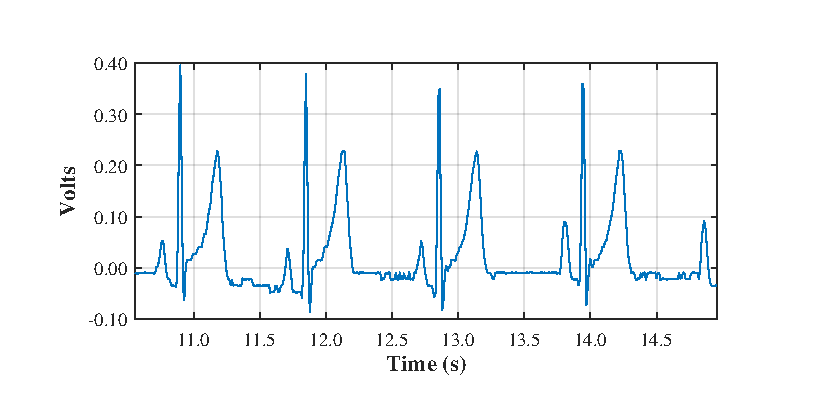
\includegraphics{figure19}    
	\caption[ECG measurement acquired by the system]{Measurement from one of the participants. Clearly, it can be identified the points P, Q, R, S and T. This signal did not change during the whole experiment.}
	\label{fig:ECG}
\end{figure} 

All the waveforms detected were typical and provided enough information about the characteristic peaks in an ECG waveform. The points P, Q, R, S and T were visible in all the signals. Nonetheless, Participant 1 showed an elevated T-wave which is presumably due to his athletic vocation. According to him, he had a ventricular hypertrophy meaning that one of his ventricles was enlarged.  

%%********************************** % Section 9.2 ******************************************
\section{Blood flow estimation from Doppler ultrasound instrument}
\label{section comparison 2}
As part of the experimental procedure, a Doppler ultrasound was used to estimate blood flow using the radial artery in the wrist as a reference. The raw data produced by the instrument came in volts which was later converted into more meaningful data using the equations \ref {eq:doppler} and \ref {eq:flow_l/min} which convert the information into units litres per minute (\si{\litre\per\minute}). As described in those equations, the angle was fixed to \SI{45}{\degree} using a laboratory support and a clamp. The cross-sectional area for calculating blood flow was the median value of~\cite {ashraf2010size}. The head of the ultrasound device was placed as close to the artery as described in the user manual of the instrument using a conductive gel as an interface between the skin and the device.

While taking the measurements, there was an electrical problem with the Doppler ultrasound instrument. Hence, it was not possible to collect data from participant 8. The data presented in figure \ref{fig:DU flow} and table \ref{tbl:DU flow} contains the results of the first seven study members.

\begin{figure}[!htb]
	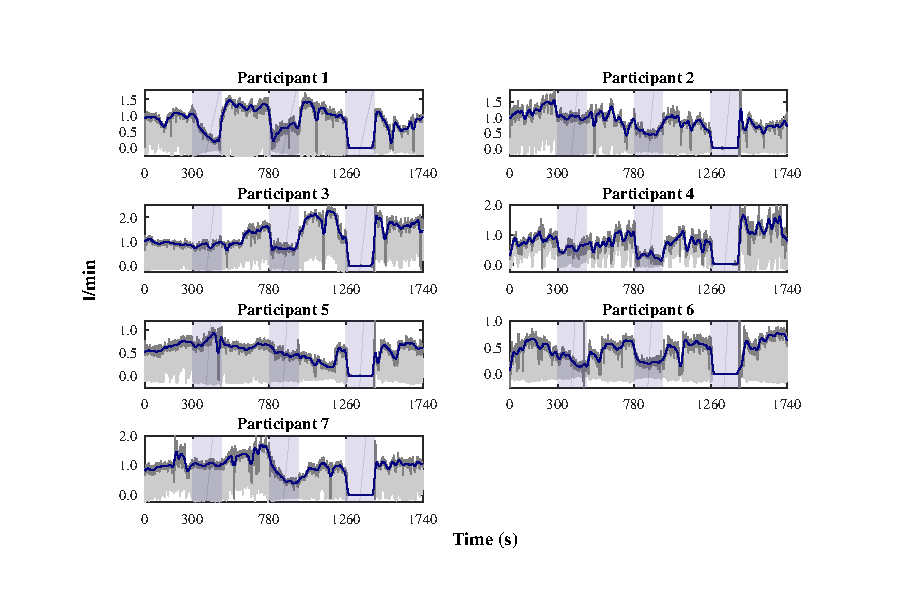
\includegraphics[width=\textwidth,keepaspectratio,trim={1cm 0cm 1.5cm 0cm},clip]{figure_cmp_2}    
	\caption[Blood flow calculated from Doppler ultrasond device all along the whole expetiment]{Blood flow calculated from the Doppler ultrasound measurements for all the participants during the experiment. The greyed out areas are the raw sign of the DU waveform. The dark blue lines represent the envelope calculated from the peak values. The blood flow was converted to the units (\si[per-mode=symbol]{\litre\per\minute}).}
	\label{fig:DU flow}
\end{figure}

%%********************************** % Section 9.2 ******************************************
\subsection{Blood flow estimation from Doppler ultrasound instrument}
\label{section comparison 2.1}
Figure \ref{fig:DU flow} shows the peak values of the Doppler ultrasound converted into the arterial flow rate. The shaded areas represent the occlusive events during the study. The measurements depict the blood flow of the radial artery and the changes during each occlusive event. During venous occlusion, it was expected not to observe a significant change of the arterial flow rate as the brachial artery was not occluded above the diastolic pressure. On the other hand, a partial arterial occlusion between diastolic a systolic pressure restricts the inflow of affecting the blood flow towards the radial artery. Finally, at the moment of occluding the brachial artery above systolic pressure, it is expected to display null blood flow.

The qualitative analysis of the DU data shows that evidently, various participants showed an alteration in their calculated median arterial flow during venous occlusion in region 2. There were different types of responses, while some experience a rapid variation within the first few seconds, in others took some time to show a resting point. More in-depth, Participant 1 evidenced an exponential flow rate decrease during this part of the test. Further, participants 2 and 4 displayed a quick drop within the first seconds followed by a settling at a mid-point. Finally, the rest of the participants did not show a significant change in flow rate during this transition. Nevertheless, the quantified data showed in \ref{tbl:DU flow} illustrated that during the transition between baseline regions 1 and 2, five out of seven participants showed a drop in their median blood flow, being Participant 1 the most obvious with a drop of \SI{52.41}{\percent} of the blood speed. The other ones exhibited a slight decrease were partakers 2,3,4 and 6 where their blood flow was about \SI{25.80(1850)}{\percent}. On the other hand, study members 5 and 7 showed a slight increase of their calculated blood flow in \SI{10.16}{\percent} and \SI{6.25}{\percent} respectively. When the cuff's pressure was released, most of the participants showed a recovery in the detected blood flow. The only ones that showed a minimal drop were participants 2 and 5.

During partial arterial occlusion, unmistakable, the arterial blood flow changed in all the participants. In this case, it is clear that the narrowing of the brachial artery restricted the blood in the arm's arterial circulation altering the flow rate speed detected by the DU. As the figure shows, most of the participants showed a quick change of blood flow as soon as the constriction was applied, excepting participant 5. In general, the reduction of the blood flow in the radial artery was about \SI{48.79(1191)}{\percent}. As soon as the flow was restored, the majority of the participants experienced an increase in their blood flood caused by a rush of blood within the arterial circulation going through a quick rush of blood for few seconds. However, participant 5 described a different response which may have been caused by the misaligned of the sensor head.  

\begin{table}[!htb]
	\caption{Mean blood flow calculated form the plethysmography wave for baseline, total occlusion and return to normality}
	\label{tbl:DU flow}
	\centering \small
	\begin{tabular}{lcccccccc}
		\toprule
		& \textbf{Region 1}
		& \textbf{Region 2}
		& \textbf{Region 3}
		& \textbf{Region 4}
		& \textbf{Region 5}
		& \textbf{Region 6}
		& \textbf{Region 7} \\
		& \textbf{[\si[per-mode=symbol]{\litre\per\minute}]}
		& \textbf{[\si[per-mode=symbol]{\litre\per\minute}]}
		& \textbf{[\si[per-mode=symbol]{\litre\per\minute}]}
		& \textbf{[\si[per-mode=symbol]{\litre\per\minute}]}
		& \textbf{[\si[per-mode=symbol]{\litre\per\minute}]}
		& \textbf{[\si[per-mode=symbol]{\litre\per\minute}]}
		& \textbf{[\si[per-mode=symbol]{\litre\per\minute}]} \\\midrule	
		Participant 1 & 0.954 & 0.430 & 1.285 & 0.618 & 1.049 & 0.003 & 0.719 \\
		Participant 2 & 1.211 & 1.014 & 0.967 & 0.546 & 0.843 & 0.002 & 0.712 \\  
		Participant 3 & 0.928 & 0.860 & 1.307 & 0.716 & 1.940 & 0.002 & 1.675 \\  
		Participant 4 & 0.826 & 0.581 & 0.764 & 0.297 & 0.754 & 0.002 & 1.245 \\  
		Participant 5 & 0.643 & 0.708 & 0.655 & 0.483 & 0.348 & 0.003 & 0.606 \\  
		Participant 6 & 0.495 & 0.248 & 0.499 & 0.230 & 0.542 & 0.002 & 0.641 \\  
		Participant 7 & 0.962 & 1.022 & 1.320 & 0.535 & 0.876 & 0.002 & 1.040 \\  	 
		\bottomrule
	\end{tabular}
\end{table}

Finally, all along with total occlusion, the tourniquet effect can be noticed in the composition of the signal with a sharp drop as soon as the occlusion took place. As expected, no arterial flow was recorded, the minimum values registered might represent artefacts in the signals. After releasing the tourniquet, all the participants experienced an increase in their flow rate to values of normality. 

%%********************************** % Section 9.3 ******************************************
\section{Measurements from Laser Doppler Flowmetry}
\label{section comparison 3}
The LDF device provided raw data in Volts which was converted into BPU units. This conversion was possible by applying equation \ref{eq:BPU} to the data collected.  As explained in section \ref{section:ldf}, the result produced is in arbitrary units which represent blood cell movement under the skin. Therefore, it illustrates the blood flow moving red blood cells in the micro-circulatory bed to distal parts of the tissue in the forearm.

Figure \ref{fig:LDF flow} displays the peaks of the LDF waveform signal in BPU. A moving average was used to aggregate 20 seconds of data to the resultant plot. That plot shows that the movement of the cell is affected when an occlusion occurs. It must be noted that a noise artefact heavily impacted some parts of the data. Such as in participants 1 and 4.

\begin{figure}[!htb]
	\centering
	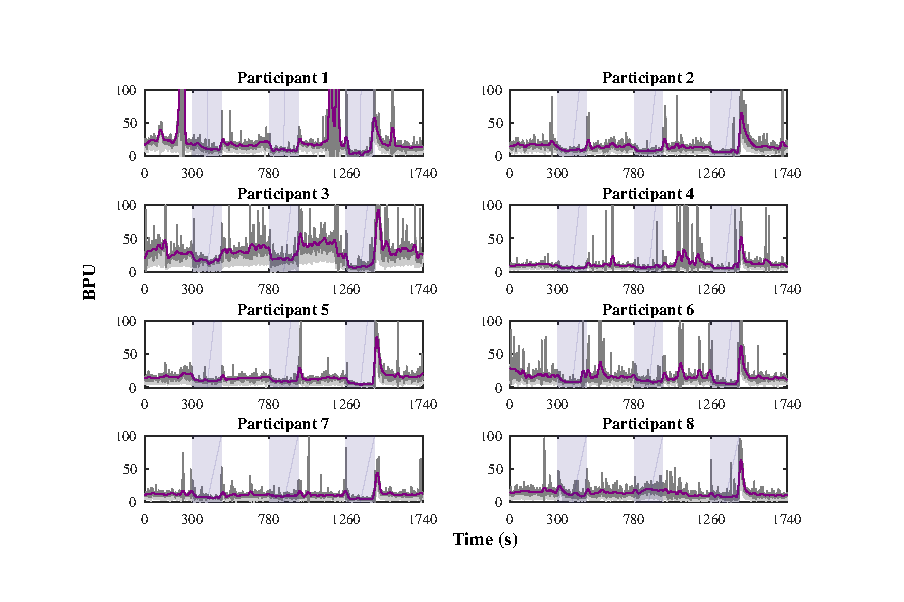
\includegraphics[width=\textwidth,keepaspectratio,trim={1cm 0cm 1.5cm 0cm},clip]{figure_cmp_3}    
	\caption[Results of the LDF in BPU]{Results of the Laser Doppler Flowmetry measurement for all the participants after being converted to BPU. The values presented in purple are equivalent to envelope signal of the peak points.}
	\label{fig:LDF flow}
\end{figure}

Nevertheless, a trend can be noticed in all the participants. During the occlusion in region 2, a slight decline in cell movement can be noticed. It shows that the venous occlusion slowed down the movement of RBC. After the cuff's pressure was released, a peak can be seen in most of the participants. This hyperaemic effect shows an acceleration of the RBC after the blockage event. 

Similar effects can be seen during partial arterial occlusion; the cells speed reduced compared to the previous baseline (region 3). Then as soon as the blockage was released, again the rush of RBCs can be detailed. Nevertheless, participant 8 seems to be an exception to the rule. His BPU tends\nknote{not sure if tends is good here} to increase slightly during the transition of region 3 to 4. Moreover, contrary to the other signals in the transition from partial arterial occlusion to baseline in region 5, his BPU decreased. These results also could explain some of the adverse readings captured by the iPG signals.

Lastly, during total occlusion, all the mean BPUs of the participants reduced considerably. Then later, when the tourniquet was released, the rush of blood flow can be noticed in the hyperaemic effect registered by the instrument, which was also detected by others instruments.

Table \ref{tbl:LDF flow} reviews the values of the mean BPU data obtained. The results declared there, are in complete agreement with the figure previously analysed.

\begin{table}[!htbp]
	\caption{Mean blood flow calculated form the plethysmography wave for baseline, total occlusion and return to normality}
	\label{tbl:LDF flow}
	\centering \small
	\begin{tabular}{lcccccccc}
		\toprule
		& \textbf{Region 1}
		& \textbf{Region 2}
		& \textbf{Region 3}
		& \textbf{Region 4}
		& \textbf{Region 5}
		& \textbf{Region 6}
		& \textbf{Region 7} \\
		& \textbf{[BPU]}
		& \textbf{[BPU]}
		& \textbf{[BPU]}		
		& \textbf{[BPU]}		
		& \textbf{[BPU]}
		& \textbf{[BPU]}
		& \textbf{[BPU]}\\\midrule
		Participant 1 & 42.89 & 12.71 & 18.37 &  9.52 & 36.44 & 11.75 & 19.64 \\  
		Participant 2 & 17.05 &  9.18 & 15.24 &  8.32 & 14.38 &  6.46 & 21.22 \\  
		Participant 3 & 30.69 & 17.08 & 33.42 & 20.72 & 40.28 &  9.27 & 38.08 \\  
		Participant 4 & 10.14 &  6.27 & 10.61 &  7.18 & 16.22 &  6.67 & 15.73 \\  
		Participant 5 & 16.66 & 10.49 & 14.16 &  9.56 & 14.58 &  5.73 & 23.70 \\  
		Participant 6 & 19.82 & 11.41 & 18.43 &  9.75 & 17.87 &  7.83 & 19.14 \\  
		Participant 7 & 12.54 &  7.45 & 11.08 &  9.32 & 10.96 &  5.91 & 14.83 \\  
		Participant 8 & 15.76 & 13.54 & 14.36 & 17.74 & 12.33 &  9.21 & 16.08 \\  
		\bottomrule
	\end{tabular}
\end{table}


%%********************************** % Section 9.4 ******************************************
\section{Measurements from the PPG Red-light signal}
\label{section comparison 4}
The PPG device provides information about the change of volume within the vascular bed under the skin. It is capable of detecting either venous or arterial blood change according to the light wavelength being used \mynote{check if this is true or find a reference}. The device employed in the experiment has an output port which provides the unprocessed raw photoplethysmography waveform. Similarly, as in the iPG signal, the PPG is composed of DC and AC parts. The DC portion of the signal is equivalent to the blood volume under the light beam. It also contains data about respiratory rate and other physiological information. On the other hand \nknote{not good use of on the other hand}, the AC component changes in amplitude synchronously according to the cardiac cycle and blood volume in the capillaries. 

During the experiment performed changes in DC and AC components can be easily identified \nknote{doesnt make sense} as showed in figure \ref{fig:RED PPG}. In the plot, the shaded regions represent each occlusive event during the test. On the left, the DC component of the PPG per participant is illustrated. This signal was obtained by detecting the low envelope values of the raw PPG waveform. In other words, the points on the foot of the waveform.  On the right-hand side is the AC component of the signal obtained by removing the low envelope of the raw data. Next, the waveform was inverted to leave only the dynamic element of the signal. Last, the peaks detected from the plethysmography waveform were redrawn in black, highlighting the maximum values during all the occlusive events.  

\begin{figure}[!htbp]
	\centering
	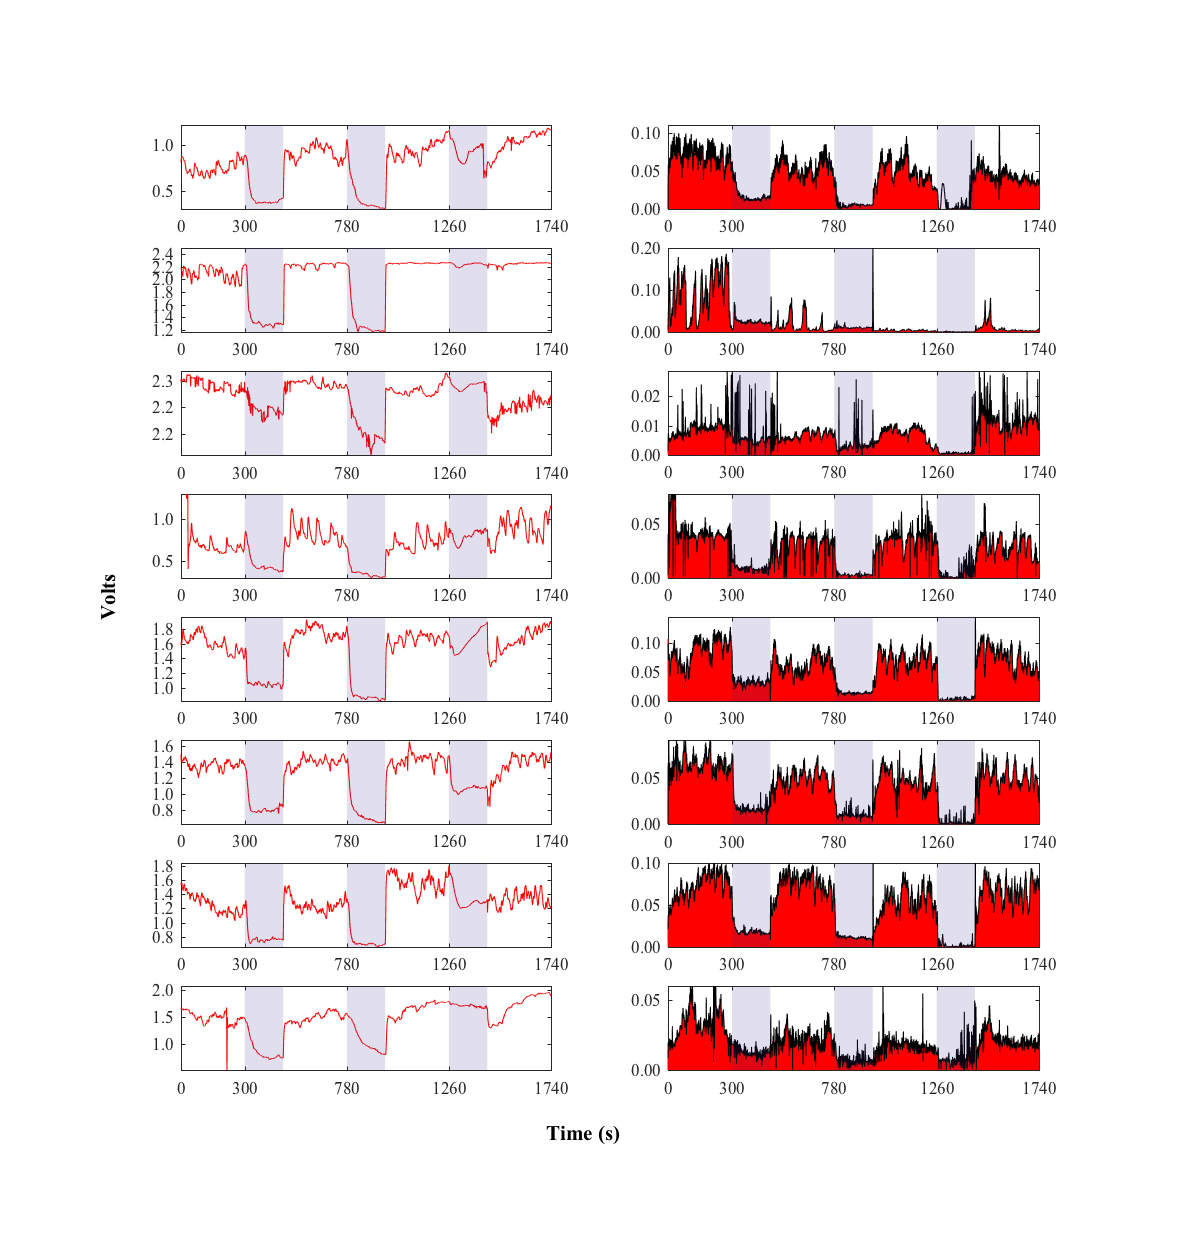
\includegraphics[width=\textwidth,keepaspectratio,trim={1cm 0cm 0cm 0 cm},clip]{figure18}    
	\caption[PPG red wavelength measurments AC and DC components]{Measurements from the red wavelength PPG sensor. On the left, the DC component of the signal, ?? it only includes the lower envelope of the waveform. On the right, the AC component of the red wavelength where the foot of the signal has been aligned to zero ??. The envelope showed in black describes the peaks of the signal}
	\label{fig:RED PPG}
\end{figure}
\nknote{??}

\begin{table}[!htbp]
	\caption[Mean peak value of the PPG DC signal for all participants in all regions]{Mean peak value of the PPG DC signal for all the participants in all the regions.}
	\label{tbl:PPG RED DC}
	\centering \small
	\begin{tabular}{lcccccccc}
		\toprule
		& \textbf{Region 1}
		& \textbf{Region 2}
		& \textbf{Region 3}
		& \textbf{Region 4}
		& \textbf{Region 5}
		& \textbf{Region 6}
		& \textbf{Region 7} \\
		& \textbf{[\si{\volt}]}
		& \textbf{[\si{\volt}]}
		& \textbf{[\si{\volt}]}		
		& \textbf{[\si{\volt}]}		
		& \textbf{[\si{\volt}]}
		& \textbf{[\si{\volt}]}
		& \textbf{[\si{\volt}]}\\\midrule
		Participant 1 & 0.75  & 0.44  & 0.91  & 0.43  & 0.94  & 0.91  & 1.03  \\  
		Participant 2 & 2.09  & 1.38  & 2.22  & 1.33  & 2.25  & 2.24  & 2.24  \\  
		Participant 3 & 2.24  & 2.20  & 2.24  & 2.16  & 2.23  & 2.24  & 2.20  \\  
		Participant 4 & 0.76  & 0.46  & 0.80  & 0.36  & 0.72  & 0.79  & 0.89  \\  
		Participant 5 & 1.60  & 1.07  & 1.73  & 0.93  & 1.66  & 1.64  & 1.64  \\  
		Participant 6 & 1.36  & 0.84  & 1.38  & 0.76  & 1.41  & 1.08  & 1.35  \\  
		Participant 7 & 1.26  & 0.79  & 1.25  & 0.75  & 1.56  & 1.32  & 1.34  \\  
		Participant 8 & 1.48  & 0.88  & 1.48  & 1.07  & 1.64  & 1.71  & 1.70  \\  
		\bottomrule
	\end{tabular}
\end{table}

From the DC signal point of view, all the participants showed a clear drop in their DC components of the signal during venous occlusion (region 2) and partial arterial occlusion (region 4). The figure clearly portrays, that the DC value dropped dramatically in most participants after the occlusive event. Nevertheless, participant 3 showed an exponential decrease in his recorded readings. Effectively, these changes can be clearly confirmed when analysing the mean values of the DC data described in Table \ref{tbl:PPG RED DC}. From there, it is calculated that the average baseline before the occlusions were \SI{1.44(055)}{\volt} for Region 1 and \SI{1.51(054)}{\volt} for Region 3. During the occlusive transitions, the DC components dropped about \SI{-0.435(0210)}{\milli\volt} and \SI{-0.528(0247)}{\milli\volt} for region 2 and region 4 respectively. Nevertheless, during total occlusion, the signals obtained were erratic with no clear shape or direction. Some participants showed a slight decrease, but others did not exhibit significant changes. In general, DC data provided valuable information during the venous and partial arterial occlusion but not conclusive results during total blood flow stoppage. 

\begin{table}[!htbp]
	\caption[Mean peak value of the PPG AC signal for all participants in all regions]{Mean peak value of the PPG AC signal for all the participants in all the regions.}
	\label{tbl:PPG RED AC}
	\centering \small
	\begin{tabular}{lcccccccc}
		\toprule
		& \textbf{Region 1}
		& \textbf{Region 2}
		& \textbf{Region 3}
		& \textbf{Region 4}
		& \textbf{Region 5}
		& \textbf{Region 6}
		& \textbf{Region 7} \\
		& \textbf{[\si{\milli\volt}]}
		& \textbf{[\si{\milli\volt}]}
		& \textbf{[\si{\milli\volt}]}		
		& \textbf{[\si{\milli\volt}]}		
		& \textbf{[\si{\milli\volt}]}
		& \textbf{[\si{\milli\volt}]}
		& \textbf{[\si{\milli\volt}]}\\\midrule
		Participant 1 & 724.83 & 180.45 & 546.76 &  66.13 & 490.87 & 109.85 & 441.54    \\  
		Participant 2 & 926.02 & 245.24 & 158.34 & 110.32 &  51.30 &   5.97 &  92.58    \\  
		Participant 3 &  94.21 &  69.72 &  68.76 &  37.19 &  71.62 &  10.54 & 122.67    \\  
		Participant 4 & 436.74 &  92.42 & 315.26 &  37.22 & 354.44 &  58.08 & 296.36    \\  
		Participant 5 & 873.38 & 324.60 & 638.53 & 155.21 & 703.81 &  51.36 & 751.62    \\  
		Participant 6 & 658.05 & 188.75 & 501.10 & 112.57 & 480.41 &  38.14 & 517.01    \\  
		Participant 7 & 731.50 & 190.43 & 746.34 & 125.76 & 547.89 &  26.92 & 660.43    \\  
		Participant 8 & 360.69 & 130.06 & 216.80 &  74.43 & 168.52 &  89.77 & 217.06    \\ 
		\bottomrule
	\end{tabular}
\end{table}

On the other hand \nknote{??use different start}, AC component produced distinctive results during each blockage event. In comparison with the DC, the AC signal was able to detect changes during total occlusion which is concurrent with the fact that there is no change of volume at that moment. Reviewing the AC signals qualitatively, participant 2 registered noisy waveforms during region 1 of the study. In addition, participant 3 had noisy peaks during the whole test, but changes through each occlusion are still visible.

From the numeric point of view, Table \ref{tbl:PPG RED AC} shows the average values of the amplitude in mV. During baseline, the mean peak value was \SI{600.67(28201)}{\milli\volt}, \SI{398.98(24421)}{\milli\volt}, \SI{358.61(23913)}{\milli\volt} and \SI{387.4073(24531)}{\milli\volt} for regions 1,3,5 and 7 respectively. In general, during venous occlusion, the signal amplitude decreased in all participants to about \SI{-422.97(21217)}{\milli\volt}. Participant 5 had the smallest change (\SI{-24.50}{\milli\volt}) compared to the rest of the signals. 

After the cuff's pressure had been released during the transition from venous occlusion to baseline, participants 2 and 3 showed an increase of their mean amplitude. The rest displayed a recovery in their signal peak to a peak of approximately \SI{221.28(21124)}{\milli\volt}. Subsequently, during partial arterial occlusion, all participants showed a decrease in their mean PPG signals amplitude, to an average of \SI{-309.14(21943)}{\milli\volt}. When comparing mean values during occlusions in region 2 and 4, the signal amplitude in region 4 was slightly lower than the one in region 2 by about \SI{-87.86(4691)}{\milli\volt}. 

Finally, during total occlusion, all the participants demonstrated a substantial decrease in their AC amplitudes. All in all, signals went below 109 mv with an average value of \SI{-48.83(3662)}{\milli\volt}.

In conclusion, the PPG waveform experienced changes of DC and AC components during each type of occlusions throughout the study. The DC signal was able to detect changes during venous and partial arterial occlusions. The difference in mean values of these two events was minimal. Nevertheless, the DC component did not show significant changes during total occlusion.  On the other hand, the AC component was able to detect changes during all occlusions. being each mean peak value significantly lowers during each test \nknote{?? improve this sentence}. 


%********************************** %Nomenclature found  *************************************
\nomenclature[z-PTT]{PTT}{Pulse transit time}